\apendice{Documentación técnica de programación}

\section{Introducción}

En este apartado se presenta la forma en que se estructura el proyecto final, el contenidos de sus directorios y ficheros, y como poder llevar a cabo la instalación y ejecución de los distintos módulos.

\section{Estructura de directorios}

%\section{Manual del programador}

\section{Compilación, instalación y ejecución del proyecto}

\subsection{Script de descarga}

Para poder ejecutar el script \texttt{mainScriptAWS.py} primero es necesario instalar las dependencias necesarias y generar el entorno de trabajo. A continuación se describen los pasos que hay que llevar a cabo para ello, mostrando los comandos que habría que usar en una máquina Debian puesto que, como ya se ha comentado, es el sistema operativo que se ha utilizado para el desarrollo del proyecto. Aún así, se debería de poder conseguir el mismo resultado en otros sistemas operativos empleando su correspondiente gestor de paquetes.

\begin{enumerate}
    \item Primero hay que instalar Python 3, \texttt{git} y \texttt{pip3} si no viene con la distribución.
\begin{verbatim}
sudo apt-get update
sudo apt-get install python3 python3-dev python3-venv
sudo apt-get install git
sudo apt-get install wget
wget https://bootstrap.pypa.io/get-pip.py
sudo python3 get-pip.py
\end{verbatim}
    
    \item El siguiente paso es crear el entorno de ejecución mediante \texttt{virtualenv}, en este caso se ha llamado \textit{testvisualenv}.
\begin{verbatim}
sudo apt-get install virtualenv
virtualenv --python=python3 testvisualenv
source testvisualenv/bin/activate
\end{verbatim}
    
    \item Después hay que instalar en nuestro entorno de trabajo las librerías y el SDK de AWS mediante \texttt{pip3}.
\begin{verbatim}
pip3 install boto3
pip3 install fs-s3fs
pip3 install git+https://github.com/Zalez95/InstaLooter.git
\end{verbatim}
    Como se puede ver, se instala el fork creado en la sección \ref{sect:descarga_publicaciones} puesto que la versión oficial de Instalooter todavía no incluye las correcciones.
    
    \item Para que Instalooter funcione hay que iniciar sesión mediante un navegador por primera vez para que se generen las cookies. Si en nuestro caso estamos empleando un sistema operativo sin navegador, entonces hay que ejecutar los siguientes pasos:
\begin{verbatim}
sudo apt-get install firefox-esr
\end{verbatim}
    Tras instalar el navegador, hay que entrar en la web de Instagram puesto que por primera vez siempre sale una ventana con un mensaje para aceptar las cookies, y tras iniciar sesión puede que salgan más ventanas para habilitar notificaciones que no son soportadas por Instalooter. Si nuestro sistema operativo no tiene interfaz gráfica como sucedió con las instancias de AWS, este proceso se tiene que hacer a través de SSH habilitando la opción de \textit{X11 Forwarding}. Para ello hay que instalar:
\begin{verbatim}
sudo apt-get install xauth x11-apps
\end{verbatim}
    Después hay que modificar el fichero \texttt{/etc/ssh/sshd\_config} y habilitar la opción \texttt{X11Forwarding yes}. Tras reiniciar, se puede conectar con la máquina virtual a través de ssh con la opción -Y para poder ejecutar aplicaciones con interfaz gráfica, en este caso con el comando \texttt{firefox} podemos lanzar el navegador y que se muestre en nuestro equipo aunque se esté ejecutando en la máquina virtual.
\end{enumerate}

Tras instalar las dependencias, el siguiente paso para poder ejecutar el script anterior es definir las siguientes variables de entorno:

\begin{itemize}
    \item \texttt{INSTA\_USER}: usuario de Instagram con el que iniciar sesión.
    \item \texttt{INSTA\_PASS}: contraseña de Instagram con el que iniciar sesión.
    \item \texttt{AWS\_AKEY\_ID}: identificador de AWS para poder usar los servicios. Este valor junto con \texttt{AWS\_AKEY\_SECRET} se puede obtener desde la web de AWS en el menú de la cuenta en \textit{Credenciales de Seguridad} > \textit{Claves de Acceso}.
    \item \texttt{AWS\_AKEY\_SECRET}: contraseña de AWS para poder usar los servicios.
\end{itemize}

Una opción para no tener que introducirlo en cada sesión es añadir las opciones anteriores al fichero \texttt{.bashrc} de la siguiente forma:

\begin{verbatim}
# ENV VARS
export INSTA_USER="..."
export INSTA_PASS="..."
export AWS_AKEY_ID="..."
export AWS_AKEY_SECRET="..."
\end{verbatim}

Por último hay que destacar que este script espera que los servicios de Amazon Web Services se estén ejecutando en \texttt{eu-west-1}, contra un bucket de Amazon S3 llamado \texttt{valltourisminstabucket} y una tabla de DynamoDB llamada \texttt{valltourisminsta}, en caso de querer emplear otras regiones, buckets o tablas habrá que modificar el script para poner los nombres correspondientes.

\subsection{Grafana y conector con DynamoDB}

Para poder crear el conector de Grafana con DynamoDB a través de las APIs REST, primero hay que generar las funciones de AWS Lambda. Para ello desde el menú principal de AWS Lambda hay que ir a \textit{Funciones} > \textit{Crear función} y crear las funciones indicadas en la sección \ref{sect:grafana_visualizacion}. El código que las implementa se encuentra en la carpeta \texttt{scripts/lambda}, tan solo hay que pegarlo en la pestaña de \textit{Código}. Todas las funciones han de tener configurado las variables de entorno \texttt{AWS\_AKEY\_ID} y \texttt{AWS\_AKEY\_SECRET} para poder acceder a DynamoDB, para ello hay que añadirlas en la pestaña \textit{Configuración} > \textit{Variables de entorno}. Una vez configuradas solo hay que darle al botón de \textit{Deploy}:

\begin{figure}[H]
    \hspace*{-2cm}
    \centering
    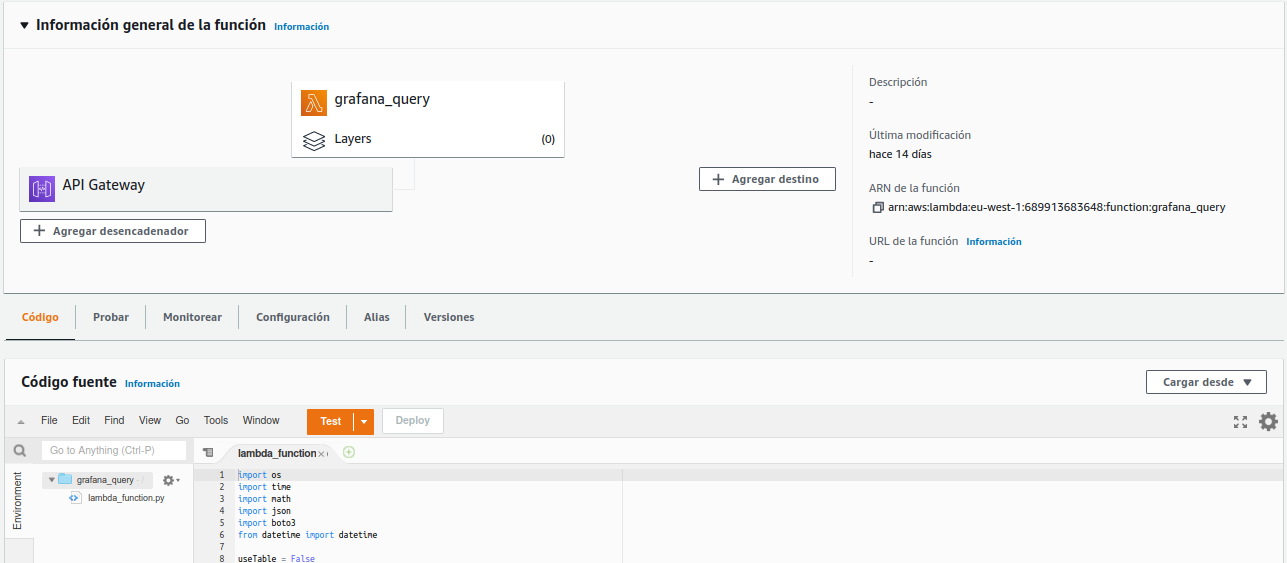
\includegraphics[width=1.2\textwidth]{memoria/img/lambda.png}
    \caption{Configuración de una función de AWS Lambda}
    \label{fig:aws_lambda}
\end{figure}

Después hay que generar las APIs REST en AWS API Gateway, para ello desde su menú en AWS hay que crear una API, en este caso llamada \textit{valltourisminsta}. Una vez creada hay que generar los recursos indicados en la sección \ref{sect:grafana_visualizacion} apuntando a las correspondientes funciones de AWS Lambda. Una vez configuradas, la API se despliega desde el menú de \textit{Acciones} > \textit{Implementar API}, en una etapa que en este caso se llamó ``demo''.

Por otro lado, una vez que se tiene el conector hay que instalar Grafana. Para ello, en un equipo Debian hay que ejecutar los siguientes comandos:

\begin{verbatim}
sudo apt-get install -y adduser libfontconfig1
wget https://dl.grafana.com/enterprise/release/grafana-
    enterprise_9.0.0_amd64.deb
sudo dpkg -i grafana-enterprise_9.0.0_amd64.deb
sudo service grafana-server start
\end{verbatim}

Tras iniciar el servicio de Grafana, éste se encontrará ejecutando en el puerto 3000, y para poder acceder solo hay que entrar mediante un navegador apuntando al equipo y puerto correspondiente. En el caso de este proyecto, como la máquina virtual que lo ejecutaba era una instancia de EC2, hubo que añadir una regla para permitir las conexiones a este puerto desde el menú de \textit{EC2} > \textit{Grupos de Seguridad}, de tipo TCP, origen \texttt{0.0.0.0/0} y puerto 3000. Tras iniciar sesión hay que instalar el plugin JSON para poder conectar a las APIs REST.

Para crear el cuadro de mandos con Grafana primero hay que crear un \textit{data source} mediante el plugin JSON que apunte a la URL de nuestro servidor en AWS API Gateway. Después desde el menu de Dashboards se crear uno nuevo. En el apartado de configuración del dashboard, existe una opción llamada llamada \textit{JSON Model}, donde si se pega el contenido del fichero \texttt{grafana\_json\_model.json} se podría obtener un cuadro de mandos idéntico al creado para este proyecto.

%\section{Pruebas del sistema}
